\documentclass[runningheads,a4paper]{llncs}

\usepackage{amssymb}
\setcounter{tocdepth}{3}
\usepackage{graphicx}

\usepackage{url}
\newcommand{\keywords}[1]{\par\addvspace\baselineskip
\noindent\keywordname\enspace\ignorespaces#1}

% Additional packages
\usepackage[utf8]{inputenc}
\usepackage[round]{natbib}
\usepackage{tikz}
\usepackage[pdftex,pdfpagelabels,bookmarks,hyperindex,hyperfigures]{hyperref}
\hypersetup{%
   plainpages=false, 
   pdfpagelayout=SinglePage,
   bookmarksopen=false,
   bookmarksnumbered=true,
   breaklinks=true,
   linktocpage,
   colorlinks=true,
   linkcolor=blue,
   urlcolor=blue,
   citecolor=blue,
   anchorcolor=green
}      

% TiKZ styles
\tikzstyle{var} = [circle,
                   thick,
                   draw, fill=red!20,
                   text width=4.5em,
                   text badly centered,
                   node distance=3cm,
                   inner sep=0pt]

\tikzstyle{factor} = [rectangle,
                      thick,
                      draw, fill=blue!20,
                      text width=1em,
                      text centered,
                      minimum height=3em,
                      minimum width=3em]

\tikzstyle{line} = [draw]

\begin{document}

\mainmatter  % start of an individual contribution

% first the title is needed
\title{Semantic Novelty Detection with Graphical Models}

% a short form should be given in case it is too long for the running head
% \titlerunning{Lecture Notes in Computer Science: Authors' Instructions}

% the name(s) of the author(s) follow(s) next
%
% NB: Chinese authors should write their first names(s) in front of
% their surnames. This ensures that the names appear correctly in
% the running heads and the author index.
%
\author{André Susano Pinto}
%
%\authorrunning{Lecture Notes in Computer Science: Authors' Instructions}
% (feature abused for this document to repeat the title also on left hand pages)

% the affiliations are given next; don't give your e-mail address
% unless you accept that it will be published
\institute{Faculdade de Engenharia da Universidade do Porto, Portugal\\
\url{andresusanopinto@gmail.com}\\
\url{http://url}}

\toctitle{Lecture Notes in Computer Science}
\tocauthor{Authors' Instructions}
\maketitle


\begin{abstract}
This papers presents an approach on implementing novelty detection at semantic level
for indoor room classification in Dora. \emph{Graphical models} are used to model
probabilistic knowledge and novelty detection is implemented on top of them.
The novelty threshold is then optimized using an unconditional probability density
model that is trained from unlabelled data.

\keywords{novelty detection, semantic data, graphical models, room classification,
indoor environments, robotics, multi-modal.}
\end{abstract}


%%%%%%%%%%%%%%%%%%%%%%%%%%%%%%%%%%%%%%%%%%%%%%%%%%%%%%%%%%%%%%%%%%%%%%
\section{Introduction}
\begin{itemize}
\item Explain context of indoor room categorization and importance of novelty detection.
\item Introduce Dora and explain how it would benefit or use the semantic novel detection.
\end{itemize}

There has been several efforts in the area of Artificial Intelligence and Robotics in creating robots
that are able to interact with humans and their environments.
One of the existing problems is a reliable high-level localization method that can be deployed into new
and unknown environments.
In this article we focus on the mapping, using \emph{semantic data}, of indoor environments such as houses and offices to room categories
such as kitchen, corridor, office.
And how to perform novelty detection on them: \emph{detect a new room category that was not present in the labelled data}.

Dora\cite{dora} (CogX: Dora) was used as a base system where this novelty detection would be implemented.
As Dora moves through the environment its \emph{conceptual layer} builds a structural and probabilistic representation of the space
instantiated as a \emph{graphical model}.
That model connects the sensed properties together with the variables used to model the world.
And allows to perform queries on the probabilities of aspects of the environment.
For example: where is most likely to find a cereal box\cite{exploiting}.

The ability to recognize novel categories on the modelled variables would allow to increase
reliability and allow the creation of self-extending behaviours.


%%%%%%%%%%%%%%%%%%%%%%%%%%%%%%%%%%%%%%%%%%%%%%%%%%%%%%%%%%%%%%%%%%%%%%
\section{Related Work}
\cite{quattoni2009recognizing} showed that most scene recognition models work poorly in indoor
scenes when compared to outdoor scenes results.
Since the properties that characterize rooms changes conforming its category. Namely corridors are
well described by global properties and bookstores are well described by the presence of specific objects (books).
Their work shows a multi-modal approach is expected to yield better performance by mixing several sources of information.

\cite{galindo2005multi} defines a bidirectional relation between object and room category, where object defines a room category and a room category provides information on where objects may be found.

Probabilistic representations are used in several localised functions in robots operating in the real-world~\cite{gross2009toomas,maierprobabilistic}. And some employ, up to some extent, a probabilistic representation across some subsystems~\cite{kraft2008exploration}.
\cite{vasudevan2008bayesian} performed room categorization through Bayesian reasoning about the presence of objects but did not included observations models (perception is considered deterministic).
And \cite{boutell2006factor} have studied outdoor scene classification using \emph{factor graphs} and modelling spatial relations between objects in the scene to extract better knowledge from semantic (high-level) features.

Its expected that using a unified probabilistic model from the whole system, such as \cite{pronobis2011exploiting}, more information can be reused to correctly predict a given random variable.

Although this paper deals with novelty detection on the robotics area, it does so using very
standard concepts and techniques such as semantic data and graphical models.
Those are often found on areas related with information retrieval.
Interesting examples are works in automatic image annotation using an hidden concept layer between visual features and text information\cite{zhang2005probabilistic}.

%%%%%%%%%%%%%%%%%%%%%%%%%%%%%%%%%%%%%%%%%%%%%%%%%%%%%%%%%%%%%%%%%%%%%%
\section{Dora Architecture Overview}
\begin{itemize}
\item Introduce Dora architecture aspects important for the paper
\item Explain what we mean by semantic data and how its captured by Dora
\item Introduce graphical models and how we use them (including notation on the paper)
\end{itemize}

Short paragraph describing dora. Short paragraph describing dora. Short paragraph describing dora. Short paragraph describing dora. Short paragraph describing dora.

From its architecture only the \emph{conceptual layer} is of interest to this article.
Its role is to aggregate the following semantic information coming from other layers:

\begin{description}
 \item[Doorway detection] is used to segment the low-level space into rooms and map connectivity between them.
 \item[Room size and shape] are classified by using 2D laser scans data and are associated as properties of a given room. The system utilizes pre-trained set of classifiers to label size as (large, medium, small) and shape as (rectangular or elongated).
 \item[Object detection] is performed using the visual input in order to detect . The system keeps track of the number of object and types seen per each room. Objects are once again detected by running a pre-trained set of detectors for: book, cereal box, computer, robot, stapler, toilet paper.
 \item[Room appearance] is categorized from the visual input by using CRFH and a pre-trained set of 7 different models.
\end{description}

With the extracted information and conceptual knowledge the conceptual layer creates a structured probabilistic representation
in order to model all known variables and their relations.
As so, in order to represent the knowledge the layer builds a \emph{chain graph}:
a probabilistic graphical model that merges both Bayesian Networks and Random Markov Fields.

The use of graphical models to describe distributions of variables has useful properties.
The edges between the variables can be seen as a kind of filter to the properties of the system.
Properties those that we expect to capture by the conceptual knowledge.
At the same time they are a generative models and therefore allow to calculate the probability
on any given subset of variables on the graph allowing the system to work even when some information is missing.


\begin{figure}[h]
\centering
\caption{The conceptual layer structures the sensed environment together with the conceptual knowledge in order to
         create a structured probabilistic representation of the world.}
\end{figure}

\subsection{Factor Graphs}
Although the conceptual layer works with \emph{chain graph}, those can be converted into \emph{factor graphs}.
We opted to use those as describing the ideas on this paper as they tend to be easier to understand.

A \emph{factor graph} is a bipartite graph connecting nodes representing random variables and factors.
Each factor represents a function dependent only on the variables to where its connected.
As so given factor graph $G$ can be seen as description of a distribution function over a set of variables obtained by
the product of all the factors. This manipulation allows to use algorithms such as the Sum-Product to efficiently calculate
probabilities on any given subset $x$ of those variables by exploiting conditional independency between variables.
We will use the notation $P_G(x)$ to represent that.

\begin{figure}[h]
\centering
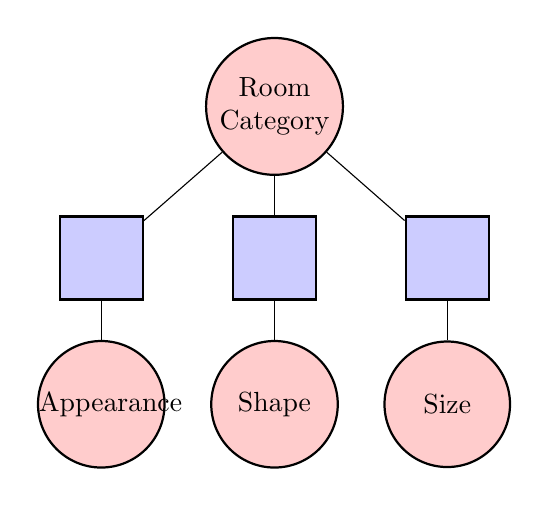
\begin{tikzpicture}[node distance = 2cm, auto]
    \matrix[row sep=0.5cm,column sep=0.5cm] {
      & \node [var] (room) {Room Category}; \\
      \node [factor] (fAppearance) {}; &
      \node [factor] (fShape) {}; &
      \node [factor] (fSize) {}; \\

      \node [var] (appearance) {Appearance}; &
      \node [var] (shape) {Shape}; &
      \node [var] (size) {Size}; \\
    };
  \path [line] (room) -- (fAppearance);
  \path [line] (room) -- (fShape);
  \path [line] (room) -- (fSize);

  \path [line] (fAppearance) -- (appearance);
  \path [line] (fShape) -- (shape);
  \path [line] (fSize) -- (size);
\end{tikzpicture}
\caption{Example of a factor graph used for Dora for representing the environment.}
\end{figure}

%%%%%%%%%%%%%%%%%%%%%%%%%%%%%%%%%%%%%%%%%%%%%%%%%%%%%%%%%%%%%%%%%%%%%%
\section{Novelty Detection}
\begin{itemize}
\item Explain 
\item Approach with a threshold function
\item Need of a normalizing factor for a threshold with dynamic functions
\item Usage of conditional density
\item Assuming of every output is equally likely
\item Using unlabelled data
\item What happens if the conditional and unconditional graphs differ only by the addition of a node?
\item How to implement that in the case a graph is a tree
\item Novelty detection on any variable of the graphical model!
\end{itemize}

Novelty detection can be performed by a threshold function sorting the input space in an optimal way to
decrease error in detection.

Its harder than a classification problem as the system only has access to positive samples.
Under that a common approach is to use conditional probability $P(x|known)$ as a threshold.

\subsection{Stable threshold}
Although in our case we are dealing with a dynamic graph $G$ that keeps changing through time as new variables
are added. Which increases the dimension of our space and spreads the distribution over the variables.

This turns it impossible to directly train a threshold function on $P_G(x)$, as we cannot assume $P(x)$ to be constant over any set of $x$.
So we need to describe $P(x)$ to develop a stable threshold on $P_G(x)/P(x)$.

A common assumption is that every possible input is equally likely then the threshold
should be $P_G(x)/(\prod |x_i|)$.

\subsection{Unlabelled data}
Nonetheless in the case of robotics its often the case we can access large amounts of unlabelled data.
This leads to an interesting point that instead of assuming a constant $P(x)$ we can actually try to build
model for it.

Under that we decided to test assuming that all probabilities are independent. That can be modelled as a graph $G'$.
And corresponding function $P_G(x)/P_{G'}(x)$.

This way our unconditional function perceive which features are slightly more biased to a certain value and will
compensate on the probability calculation.

This step is important to achieve a correct order of the input space.


%%%%%%%%%%%%%%%%%%%%%%%%%%%%%%%%%%%%%%%%%%%%%%%%%%%%%%%%%%%%%%%%%%%%%%
\section{Results}
\begin{itemize}
\item Show results and how much it improves by using a simple method for unconditional probability
\end{itemize}

%%%%%%%%%%%%%%%%%%%%%%%%%%%%%%%%%%%%%%%%%%%%%%%%%%%%%%%%%%%%%%%%%%%%%%
\section{Conclusions and Future Work}
\begin{itemize}
\item Show a correct estimation of unconditional probability to be important in estabilishing a novelty detection threshold
\item Show unlabelled data can be used for it.
\item Although focus on Room Categorization we expect the results and techniques to be usable on other areas.
\end{itemize}

%%%%%%%%%%%%%%%%%%%%%%%%%%%%%%%%%%%%%%%%%%%%%%%%%%%%%%%%%%%%%%%%%%%%%%
\bibliographystyle{plainnat}
\bibliography{refs}

\end{document}
